
— Fiuuuuuuu... Ssssssssssssssssss... Ploc Ploc Ploc....
\bigbreak
Hoje começa a Primavera.
\bigbreak
Estamos num jardim de uma casinha pequena e muito arrumada, mas com um espaço enorme à sua volta.

Não tem grades nem muros.

Também não é preciso, pois nesta morada tudo é simples e apenas se sabe onde acaba o jardim e começa a estrada, porque as árvores cresceram posicionadas como guardiãs e porteiras de boas vindas.

São árvores altas, de tronco forte, com copas majestosas e ramos abertos para o céu e para os lados. Parecem braços a querer abraçar quem passa.

O jardim... ai como este jardim é bonito!

Tapetado de relva muito verde e bem cuidada.

Nele crescem canteiros de flores de todas as cores, assim como flores de todas as espécies. Grandes, pequenas, pequeníssimas, com pétalas, com cálices, com cachos, com picos, sem picos.
Algumas das flores têm nomes de pessoas. Ou serão as pessoas que têm nome de flor? Margarida, Rosa, Flora, Hortência, Íris, Flor.
As árvores não ficam de fora nessa miscelânea e apelidos são dados às criaturas humanas para que não se esqueçam delas: Oliveira, Carvalho, Pereira, Macieira, Pinheiro. Neste jardim tudo se confunde.

A disposição natural do Reino Vegetal é primorosa.

A casinha fica colocada no centro do jardim e está rodeada por 24 canteiros e estes distanciam-se dela uns 12 passos largos. E as árvores guardiãs crescem num segundo círculo, distanciando-se também uns 12 passos das flores. São 48 sentinelas, sempre observando tudo o que entra e sai do jardim, por terra e pelo ar.
\bigbreak
O sol eleva-se neste preciso momento por detrás das copas das árvores e ilumina todos os cantos e recantos deste lugar.

As sombras transmutam-se em luz e o relvado muda de cor verde escura para verde resplandecente.

Tudo brilha, tudo está luminoso.

Tem início um movimento discreto, bem debaixo dos canteiros das flores.

Começam a sair pequenos insetos das suas tocas, que bocejam e se espreguiçam, dando um bom dia ao sol.

E no céu voam os passarinhos que saíram dos seus ninhos e que dançam em alegria.

Cantam e gorjeiam, acordando tudo e todos.
O dia começou!

Hoje começa a Primavera.
\bigbreak
— Fiuuuuuuu... Ssssssssssssssssss... Ploc Ploc Ploc....

\begin{figure}[h]
    \centering
    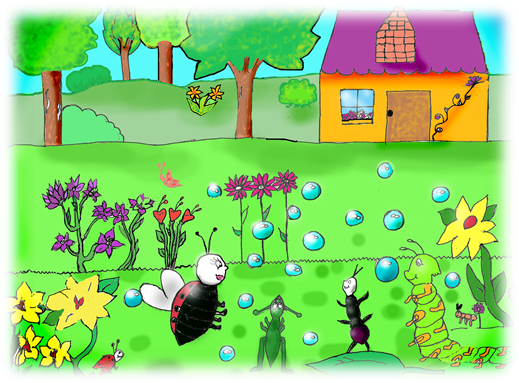
\includegraphics[width=0.75\textwidth]{jardim}
\end{figure}


Sente-se uma brisa suave e um monte de bolinhas, parecidas com bolas de sabão, invadem o ar do jardim vindas de lugar nenhum. São de todas as cores e algumas têm vários tons, assemelhando-se a um arco-íris.

Quando tocam o chão, Ploc Ploc Ploc, desaparecem no nada.

— Olhem que bolinhas estranhas! – diz uma lagarta que rasteja apressada para chegar a uma das bolas que pousou perto de si. Mas chegou atrasada, porque a bolinha fez Ploc.

— São lindas! E são tantas! – o gafanhoto dá um grande salto na esperança de apanhar uma.

— Devem ter estado a lavar roupa no céu! – sussurra uma joaninha, tentando encontrar uma lógica para o acontecimento.
\bigbreak
Os insetos estão boquiabertos e sem saber o que pensar. No seu jardim está a nevar… bolas de sabão.
\bigbreak
— Fiuuuuuu.... um vento muito fresco faz esvoaçar as bolas no ar.

Como são seres organizados e muito conscientes do seu jardim, quando alguma coisa fora do comum acontece, reúnem-se sempre e como de costume, em Unidade, debaixo do canteiro dos lírios.

Aquele foi, é e sempre será o canteiro das reuniões.

Exércitos de formigas, mãos cheias de joaninhas, braçadas de gafanhotos e um monte de lagartas esperam junto aos lírios, na esperança de que algumas das bolinhas tombem perto de si.

Uma bola de sabão começa a flutuar na direção deles. Ora vai para a direita, ora vai para a esquerda, agora sobe, depois desce e, quando está quase a cair e fazer Ploc, isso não acontece e ela volta a subir.

Os olhinhos dos insetos ali presentes percorrem o trajeto da misteriosa bola.

E em uníssono vão murmurando:
\bigbreak
— Oooooooh! Eh! Iiiih! Uh! Aaaaaaaah!
\bigbreak
Então, uma surpresa acontece.